%===============================================================================
% zentrale Layout-Angaben und Befehle
%===============================================================================
%
\RequirePackage{ifpdf}
\ifpdf
\documentclass[pdftex, a4paper, 12pt]{article}
\else
\documentclass[a4paper, 12pt]{article}
\fi
\usepackage{german}
\usepackage[latin1]{inputenc}
\usepackage{fancyhdr}
\usepackage[T1]{fontenc}
\usepackage{ae}
\usepackage{listings}
\usepackage{color}
%
\ifpdf
\usepackage[pdftex,bookmarksopen,bookmarksnumbered,pdfborder=0]{hyperref}
\usepackage[pdftex]{graphicx}
\pdfcompresslevel=9
\else
\usepackage{url}
\usepackage[dvips]{graphicx}
\fi
%
% ausf�hrlichere Fehlermeldungen
\errorcontextlines=999
%
% Page-Layout
\setlength\headheight{14pt}
\setlength\topmargin{-15,4mm}
\setlength\oddsidemargin{-10mm}
\setlength\evensidemargin{-10mm}
\setlength\textwidth{180mm}
\setlength\textheight{252mm}
%
% Absatzeinstellungen
\setlength\parindent{0mm}
\setlength\parskip{2ex}
%
% Anweisung zur Erstellung der Titelseite
% #1 = Name der Diplomarbeit
% #2 = Autor
% #3 = Abgabedatum
% #4 = Autor
\renewcommand{\maketitle}[4]
{\begin{titlepage}
\centering
\begin{minipage}[t]{18cm}
\begin{minipage}{3cm}
    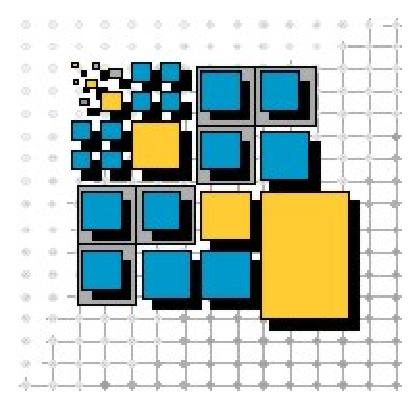
\includegraphics[height=26mm]{include/logo}
\end{minipage}
\hfill
\begin{minipage}{11,5cm}
  \centering
    Otto-Friedrich-Universit\"at Bamberg\\[12pt]
    {\Large Distributed and Mobile Systems Group}
\end{minipage}
\hfill
\begin{minipage}{3cm}
    
\includegraphics[height=26mm]{include/uni}
\end{minipage}
\end{minipage}\\[170pt]
%Zum Thema:\\[24pt]
{\Huge #1}\\[12pt]
{\Huge User's Manual}\\
\vfill
\begin{minipage}{\textwidth}
%\center
%Vorgelegt von:\\
#2\\
#4\\[18pt]
Lehrstuhl f\"ur Praktische Informatik \\
Otto-Friedrich-Universit\"at Bamberg\\
Feldkirchenstr. 21\\
D-96052 Bamberg\\
GERMANY
\\[12pt]
#3\\
\end{minipage}
\end{titlepage}
}% wird fr Hintergrund von Code bentigt
\definecolor{hellgrau}{gray}{0.9}
%
% Einstellungen fr Java-Code
\lstdefinestyle{javaStyle}{%
  basicstyle=\ttfamily,%
  backgroundcolor=\color{hellgrau},%
  keywordstyle=\itshape,%
  tabsize=2,
  showstringspaces=false,%
  language=Java,%
  numbers=left,%
  numberstyle=\tiny,%
  stepnumber=1,%
  numbersep=5pt,%
  extendedchars=true,%
  xleftmargin=1em,%
  lineskip=-1pt,%
  breaklines%
}
%
% neues environment fr Java-Sourcecode
% #1 = "caption={Hier eigene �erschrift}, label={Hier eigenes Label}"
\lstnewenvironment{javacode}[1][]{%
\lstset{style=javaStyle,#1}%
}{}
%
% Befehl zum Einbinden von Java-Sourcecode aus Datei
% #1 = Dateiname relativ zu src-Verzeichnis
% #2 = �erschrift
% #3 = Label
\newcommand{\javafile}[3]{%
\vspace{-0.5cm}
\begin{center}
   \lstinputlisting[%
     caption={#2},%
     label={#3},%
     style=javaStyle]{src/#1}%
\end{center}
\vspace{-0.5cm}
}
%
%
% setzen von kopf und fusszeile
\newcommand{\settopbottom}
{
  \fancyhf{}
  \fancyhead[LO]{\footnotesize\sc\nouppercase{\leftmark}}
  \fancyhead[RO]{\footnotesize\sc\nouppercase{\rightmark}}
  \fancyfoot[LO]{\footnotesize\sc Lehrstuhl f�r Praktische Informatik}
  \fancyfoot[RO]{\thepage}
  \renewcommand{\headrulewidth}{0pt}
  \renewcommand{\footrulewidth}{0pt}
}
%
% setzen nur von fusszeile
\newcommand{\setbottom}
{
  \pagestyle{fancy}
  \fancyhf{}
  \fancyfoot[LO]{\footnotesize\sc Lehrstuhl f�r Praktische Informatik}
  \fancyfoot[RO]{\thepage}
  \renewcommand{\headrulewidth}{0pt}
  \renewcommand{\footrulewidth}{0pt}
}
%
% Erstellung von Abk�rzungsverzeichnis
\newcommand{\abbrev}[2]{#1 & #2\\}
\newcommand{\abkuerzungen}{
\section*{List of abbreviations}
\hspace{2ex}
\begin{tabular}{ll}
\input{abkuerzungen.tex}
\end{tabular}
}
%
% Einbindung eines Bildes mit angegebener Breite
% #1 = label f�r \ref-Verweise
% #2 = Name des Bildes ohne Endung relativ zu images-Verzeichnis
% #3 = Beschriftung
% #4 = Breite des Bildes im Dokument in cm
\newcommand{\bildw}[4]{%
  \begin{figure}[htb]%
    \centering%
    \includegraphics[width=#4cm]{images/#2}%
    \vskip -0.3cm%
    \caption{#3}%
    \vskip -0,2cm%
    \label{#1}%
  \end{figure}%
}
%
% Einbindung eines Bildes mit Seitenbreite
% #1 = label f�r \ref-Verweise
% #2 = Name des Bildes ohne Endung relativ zu images-Verzeichnis
% #3 = Beschriftung
\newcommand{\bild}[3]{%
  \begin{figure}[htb]%
    \centering%
    \includegraphics[width=\textwidth]{images/#2}%
    \vskip -0.3cm%
    \caption{#3}%
    \vskip -0,2cm%
    \label{#1}%
\end{figure}%
}
